
\section{Introduction}

In the previous Chapters I studied the effect that adding positive feedback loops to the genetic toggle switch has on the robustness of the system. In this Chapter I provide the experimental design for the construction of the genetic toggle switch with single and double positive autoregulation in the lab. 

Structurally, this Chapter is organised as follows: First I provide an overview of the cloning plan, by listing the relevant BioBrick parts used and their interactions. Then I outline the methods that are used during the cloning procedure and finally I provide the experimental design for producing these switches.


\section{Cloning overview}


\begin{figure*}[t]
	\begin{center}
		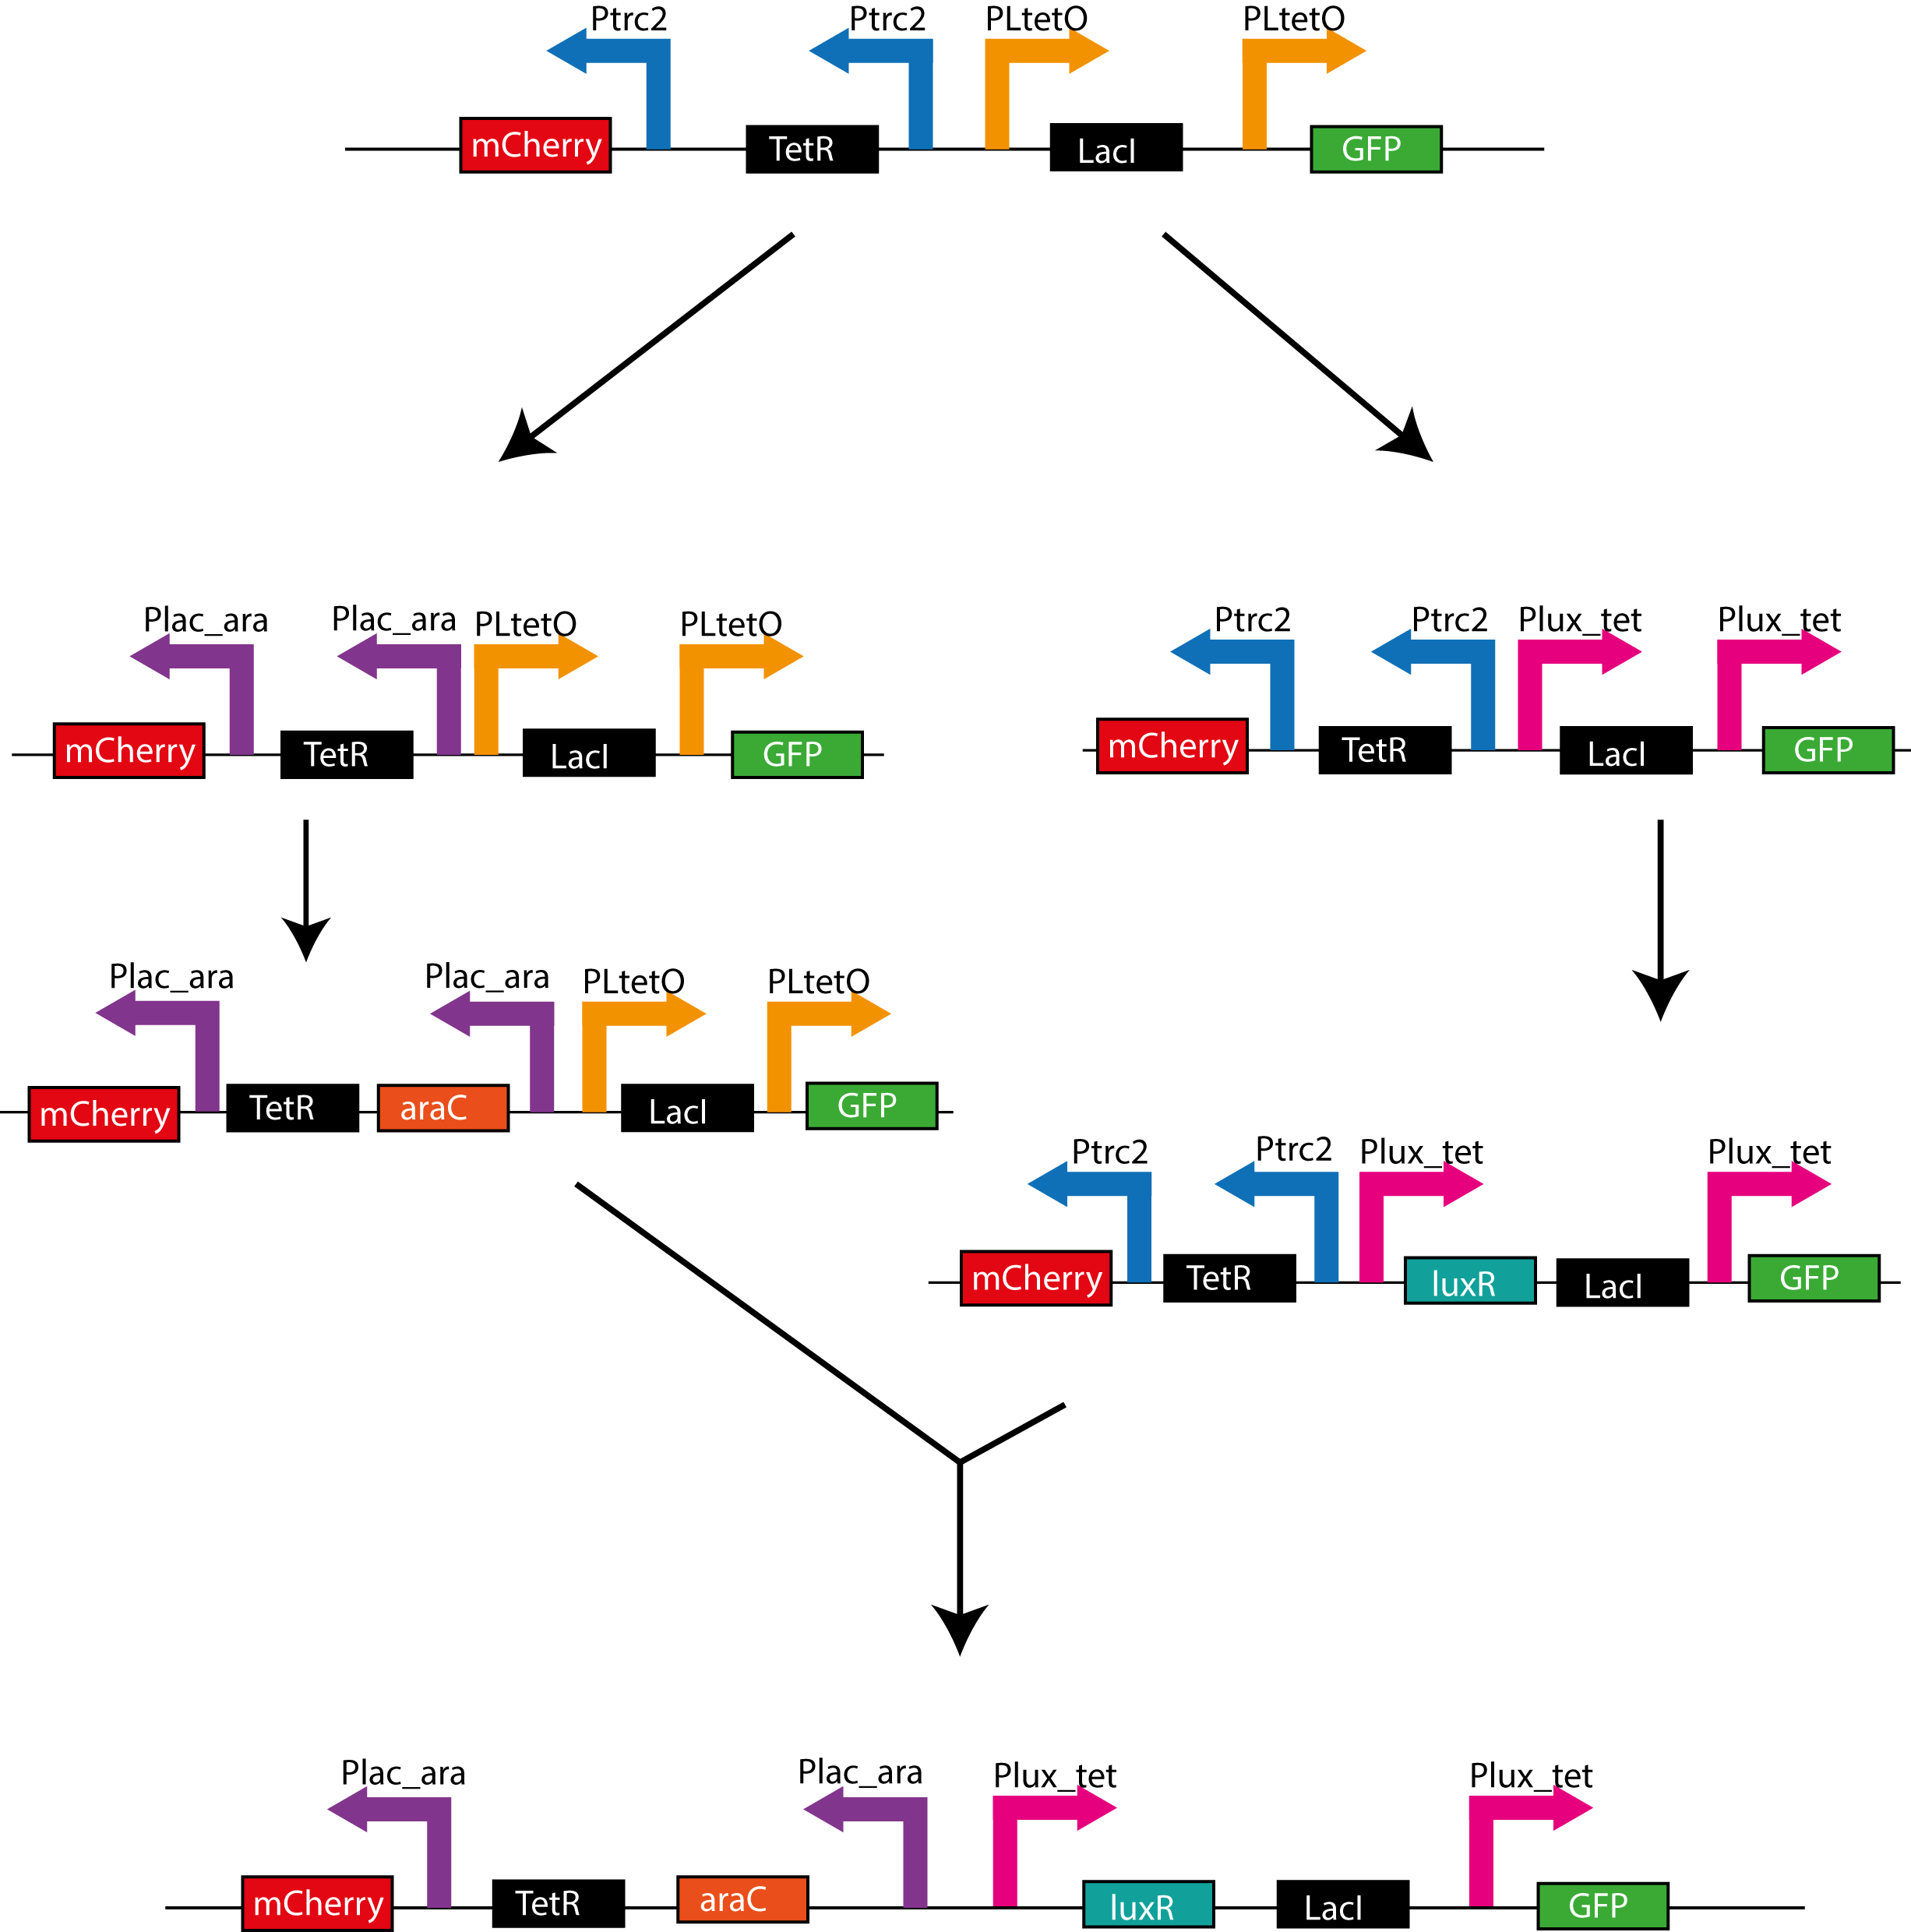
\includegraphics[scale=0.7]{../../chapters/chapterDesignSwitches/images/switches_cloning_big.png}
		\caption[LoF caption]{\label{fig:plan}}
	\end{center}
\end{figure*}
\clearpage

\section{Experimental design}



\begin{figure*}[t]
	\begin{center}
		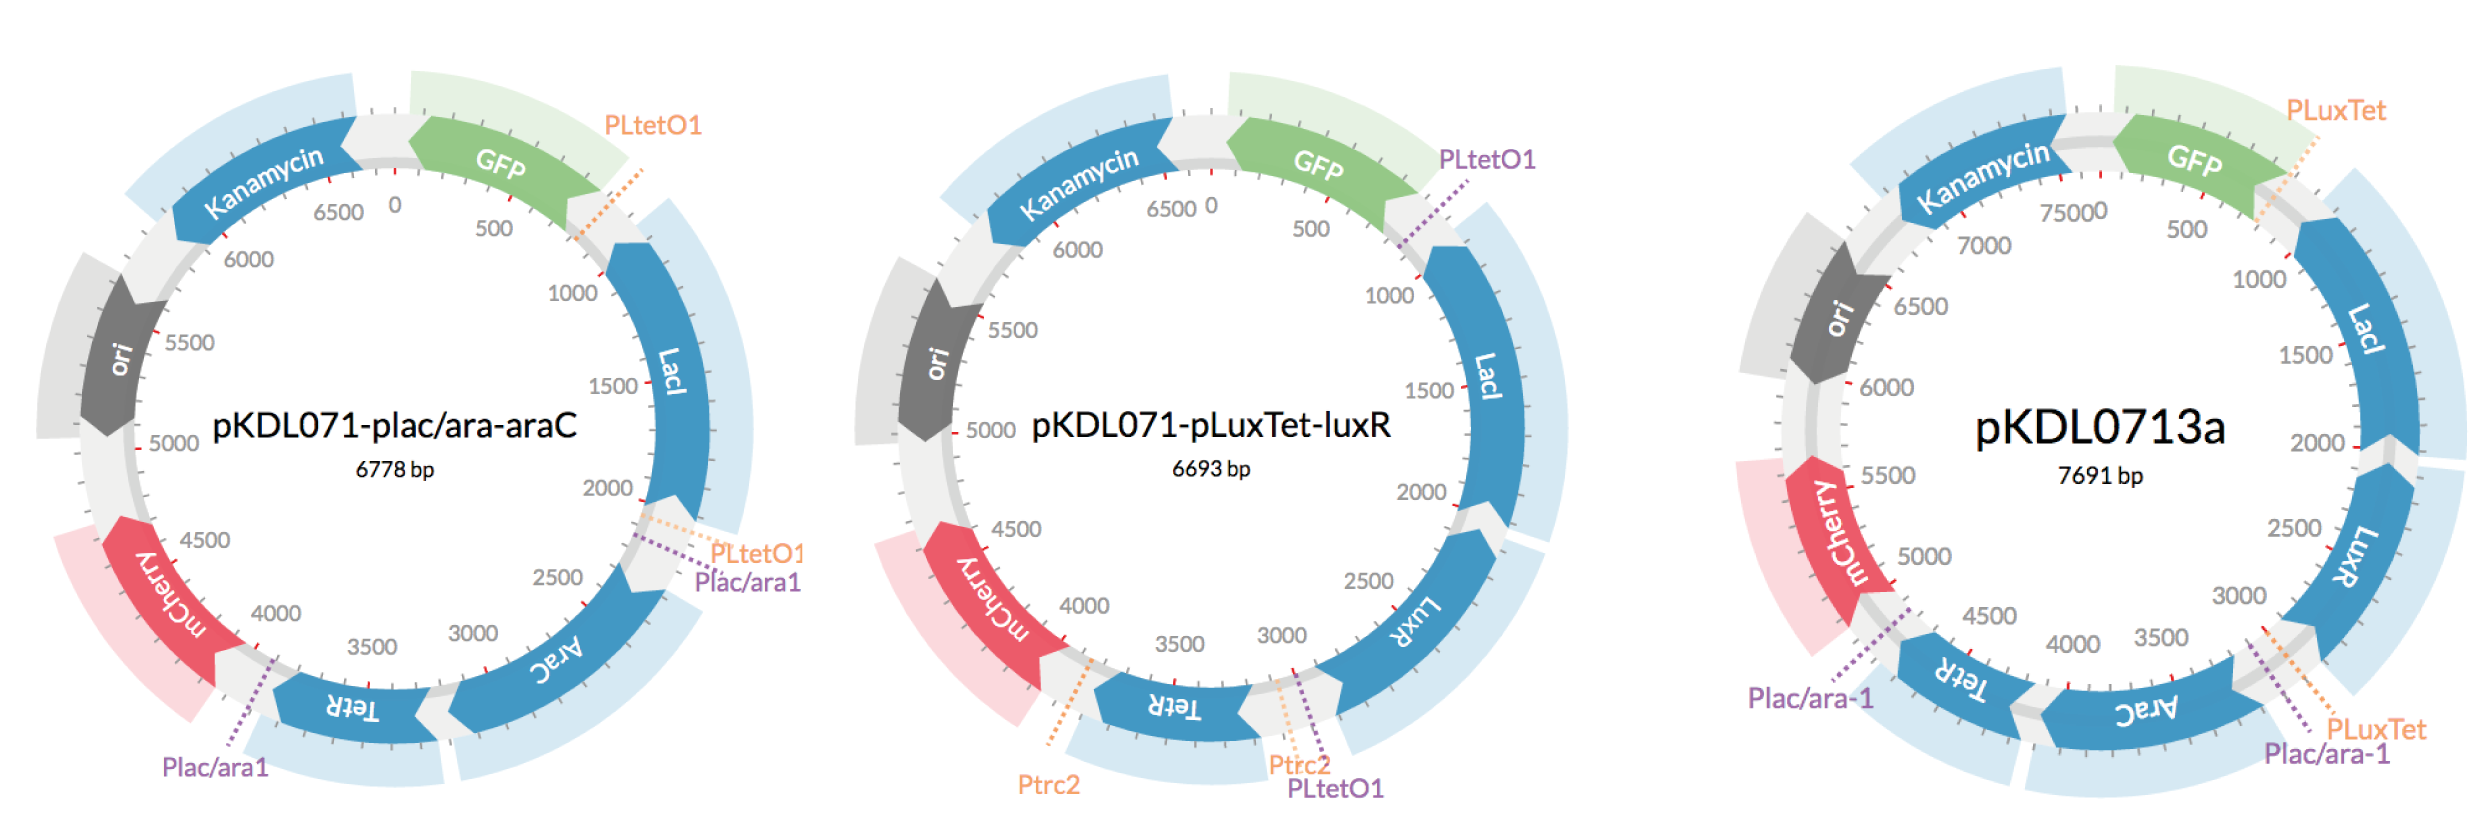
\includegraphics[scale=0.7]{../../chapters/chapterDesignSwitches/images/final-plasmids.png}
		\caption[LoF caption]{\label{fig:finalpl}}
	\end{center}
\end{figure*}
